\documentclass{standalone}
\usepackage{tikz}
\usetikzlibrary{patterns, positioning}


\begin{document}
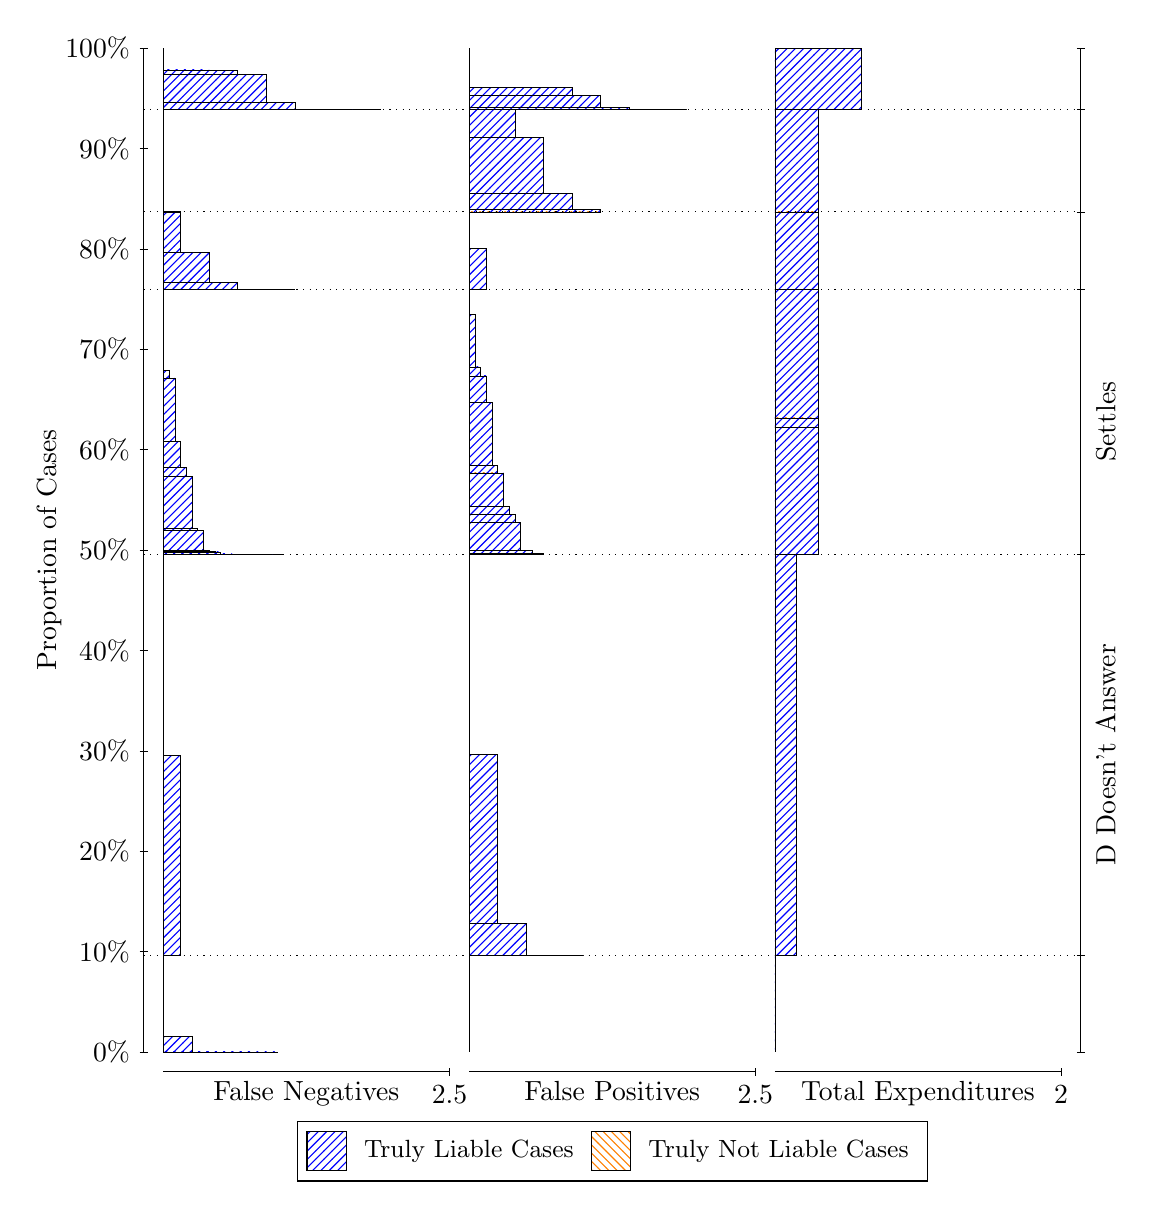
\begin{tikzpicture}
\draw[black, very thin] (1.5,1.75) -- (1.5,14.5);
\node[rotate=90, text=black, anchor=center] at (0.3, 8.125) {Proportion of Cases};
\draw[black, very thin] (1.45,1.75) -- (1.55,1.75);
\node[text=black, anchor=east] at (1.45, 1.75) {0\%};
\draw[black, very thin] (1.45,3.025) -- (1.55,3.025);
\node[text=black, anchor=east] at (1.45, 3.025) {10\%};
\draw[black, very thin] (1.45,4.3) -- (1.55,4.3);
\node[text=black, anchor=east] at (1.45, 4.3) {20\%};
\draw[black, very thin] (1.45,5.575) -- (1.55,5.575);
\node[text=black, anchor=east] at (1.45, 5.575) {30\%};
\draw[black, very thin] (1.45,6.85) -- (1.55,6.85);
\node[text=black, anchor=east] at (1.45, 6.85) {40\%};
\draw[black, very thin] (1.45,8.125) -- (1.55,8.125);
\node[text=black, anchor=east] at (1.45, 8.125) {50\%};
\draw[black, very thin] (1.45,9.4) -- (1.55,9.4);
\node[text=black, anchor=east] at (1.45, 9.4) {60\%};
\draw[black, very thin] (1.45,10.675) -- (1.55,10.675);
\node[text=black, anchor=east] at (1.45, 10.675) {70\%};
\draw[black, very thin] (1.45,11.95) -- (1.55,11.95);
\node[text=black, anchor=east] at (1.45, 11.95) {80\%};
\draw[black, very thin] (1.45,13.225) -- (1.55,13.225);
\node[text=black, anchor=east] at (1.45, 13.225) {90\%};
\draw[black, very thin] (1.45,14.5) -- (1.55,14.5);
\node[text=black, anchor=east] at (1.45, 14.5) {100\%};

\draw[black, very thin] (13.4,1.75) -- (13.4,14.5);
\draw[black, very thin] (13.35,1.75) -- (13.45,1.75);
\node[anchor=west] at (13.35, 1.75) {};
\draw[black, very thin] (13.35,2.9732) -- (13.45,2.9732);
\node[anchor=west] at (13.35, 2.9732) {};
\draw[black, very thin] (13.35,8.0714) -- (13.45,8.0714);
\node[anchor=west] at (13.35, 8.0714) {};
\draw[black, very thin] (13.35,11.437) -- (13.45,11.437);
\node[anchor=west] at (13.35, 11.437) {};
\draw[black, very thin] (13.35,12.419) -- (13.45,12.419);
\node[anchor=west] at (13.35, 12.419) {};
\draw[black, very thin] (13.35,13.721) -- (13.45,13.721);
\node[anchor=west] at (13.35, 13.721) {};
\draw[black, very thin] (13.35,14.5) -- (13.45,14.5);
\node[anchor=west] at (13.35, 14.5) {};

\draw[black, very thin, pattern color=blue, pattern=north east lines] (1.75,1.75) rectangle (3.2033,1.75);
\draw[black, very thin, pattern color=blue, pattern=north east lines] (1.75,1.75) rectangle (2.84,1.75);
\draw[black, very thin, pattern color=blue, pattern=north east lines] (1.75,1.75) rectangle (2.4767,1.7517);
\draw[black, very thin, pattern color=blue, pattern=north east lines] (1.75,1.7517) rectangle (2.1133,1.9503);
\draw[black, very thin, pattern color=orange, pattern=north west lines] (1.75,1.9503) rectangle (1.75,1.9503);
\draw[black, very thin, pattern color=blue, pattern=north east lines] (1.75,1.9503) rectangle (1.75,2.9732);
\draw[black, very thin, pattern color=blue, pattern=north east lines] (1.75,2.9732) rectangle (1.968,5.519);
\draw[black, very thin, pattern color=orange, pattern=north west lines] (1.75,5.519) rectangle (1.75,5.519);
\draw[black, very thin, pattern color=blue, pattern=north east lines] (1.75,5.519) rectangle (1.75,8.0714);
\draw[black, very thin, pattern color=blue, pattern=north east lines] (1.75,8.0714) rectangle (3.276,8.0714);
\draw[black, very thin, pattern color=blue, pattern=north east lines] (1.75,8.0714) rectangle (3.1307,8.0714);
\draw[black, very thin, pattern color=blue, pattern=north east lines] (1.75,8.0714) rectangle (2.9853,8.0714);
\draw[black, very thin, pattern color=blue, pattern=north east lines] (1.75,8.0714) rectangle (2.9127,8.0714);
\draw[black, very thin, pattern color=blue, pattern=north east lines] (1.75,8.0714) rectangle (2.84,8.0714);
\draw[black, very thin, pattern color=blue, pattern=north east lines] (1.75,8.0714) rectangle (2.7673,8.0714);
\draw[black, very thin, pattern color=blue, pattern=north east lines] (1.75,8.0714) rectangle (2.6947,8.0714);
\draw[black, very thin, pattern color=blue, pattern=north east lines] (1.75,8.0714) rectangle (2.622,8.076);
\draw[black, very thin, pattern color=blue, pattern=north east lines] (1.75,8.076) rectangle (2.5493,8.0764);
\draw[black, very thin, pattern color=blue, pattern=north east lines] (1.75,8.0764) rectangle (2.4767,8.102);
\draw[black, very thin, pattern color=blue, pattern=north east lines] (1.75,8.102) rectangle (2.404,8.1105);
\draw[black, very thin, pattern color=blue, pattern=north east lines] (1.75,8.1105) rectangle (2.3313,8.126);
\draw[black, very thin, pattern color=blue, pattern=north east lines] (1.75,8.126) rectangle (2.2587,8.3697);
\draw[black, very thin, pattern color=blue, pattern=north east lines] (1.75,8.3697) rectangle (2.186,8.3959);
\draw[black, very thin, pattern color=blue, pattern=north east lines] (1.75,8.3959) rectangle (2.1133,9.0574);
\draw[black, very thin, pattern color=blue, pattern=north east lines] (1.75,9.0574) rectangle (2.0407,9.173);
\draw[black, very thin, pattern color=blue, pattern=north east lines] (1.75,9.173) rectangle (1.968,9.5083);
\draw[black, very thin, pattern color=blue, pattern=north east lines] (1.75,9.5083) rectangle (1.8953,10.31);
\draw[black, very thin, pattern color=blue, pattern=north east lines] (1.75,10.31) rectangle (1.8227,10.404);
\draw[black, very thin, pattern color=orange, pattern=north west lines] (1.75,10.404) rectangle (1.75,10.404);
\draw[black, very thin, pattern color=blue, pattern=north east lines] (1.75,10.404) rectangle (1.75,11.437);
\draw[black, very thin, pattern color=blue, pattern=north east lines] (1.75,11.437) rectangle (3.4213,11.437);
\draw[black, very thin, pattern color=blue, pattern=north east lines] (1.75,11.437) rectangle (3.058,11.439);
\draw[black, very thin, pattern color=blue, pattern=north east lines] (1.75,11.439) rectangle (2.6947,11.528);
\draw[black, very thin, pattern color=blue, pattern=north east lines] (1.75,11.528) rectangle (2.3313,11.905);
\draw[black, very thin, pattern color=blue, pattern=north east lines] (1.75,11.905) rectangle (1.968,12.419);
\draw[black, very thin, pattern color=orange, pattern=north west lines] (1.75,12.419) rectangle (1.75,12.419);
\draw[black, very thin, pattern color=blue, pattern=north east lines] (1.75,12.419) rectangle (1.968,12.423);
\draw[black, very thin, pattern color=orange, pattern=north west lines] (1.75,12.423) rectangle (1.75,12.423);
\draw[black, very thin, pattern color=blue, pattern=north east lines] (1.75,12.423) rectangle (1.75,13.721);
\draw[black, very thin, pattern color=blue, pattern=north east lines] (1.75,13.721) rectangle (4.5113,13.721);
\draw[black, very thin, pattern color=blue, pattern=north east lines] (1.75,13.721) rectangle (4.148,13.721);
\draw[black, very thin, pattern color=blue, pattern=north east lines] (1.75,13.721) rectangle (3.7847,13.724);
\draw[black, very thin, pattern color=blue, pattern=north east lines] (1.75,13.724) rectangle (3.4213,13.813);
\draw[black, very thin, pattern color=blue, pattern=north east lines] (1.75,13.813) rectangle (3.058,14.169);
\draw[black, very thin, pattern color=blue, pattern=north east lines] (1.75,14.169) rectangle (2.6947,14.22);
\draw[black, very thin, pattern color=blue, pattern=north east lines] (1.75,14.22) rectangle (2.404,14.22);
\draw[black, very thin, pattern color=blue, pattern=north east lines] (1.75,14.22) rectangle (2.3313,14.221);
\draw[black, very thin, pattern color=blue, pattern=north east lines] (1.75,14.221) rectangle (2.0407,14.221);
\draw[black, very thin, pattern color=orange, pattern=north west lines] (1.75,14.221) rectangle (1.75,14.221);
\draw[black, very thin, pattern color=blue, pattern=north east lines] (1.75,14.221) rectangle (1.75,14.5);
\draw[black, very thin, pattern color=orange, pattern=north west lines] (5.6333,1.75) rectangle (5.6333,1.75);
\draw[black, very thin, pattern color=blue, pattern=north east lines] (5.6333,1.75) rectangle (5.6333,2.9732);
\draw[black, very thin, pattern color=orange, pattern=north west lines] (5.6333,2.9732) rectangle (7.0867,2.9732);
\draw[black, very thin, pattern color=blue, pattern=north east lines] (5.6333,2.9732) rectangle (7.0867,2.9732);
\draw[black, very thin, pattern color=blue, pattern=north east lines] (5.6333,2.9732) rectangle (6.7233,2.9763);
\draw[black, very thin, pattern color=blue, pattern=north east lines] (5.6333,2.9763) rectangle (6.36,3.3807);
\draw[black, very thin, pattern color=blue, pattern=north east lines] (5.6333,3.3807) rectangle (5.9967,5.5256);
\draw[black, very thin, pattern color=blue, pattern=north east lines] (5.6333,5.5256) rectangle (5.6333,8.0714);
\draw[black, very thin, pattern color=orange, pattern=north west lines] (5.6333,8.0714) rectangle (6.578,8.0714);
\draw[black, very thin, pattern color=blue, pattern=north east lines] (5.6333,8.0714) rectangle (6.578,8.0818);
\draw[black, very thin, pattern color=orange, pattern=north west lines] (5.6333,8.0818) rectangle (6.4327,8.0818);
\draw[black, very thin, pattern color=blue, pattern=north east lines] (5.6333,8.0818) rectangle (6.4327,8.1192);
\draw[black, very thin, pattern color=orange, pattern=north west lines] (5.6333,8.1192) rectangle (6.2873,8.1192);
\draw[black, very thin, pattern color=blue, pattern=north east lines] (5.6333,8.1192) rectangle (6.2873,8.4805);
\draw[black, very thin, pattern color=blue, pattern=north east lines] (5.6333,8.4805) rectangle (6.2147,8.5797);
\draw[black, very thin, pattern color=orange, pattern=north west lines] (5.6333,8.5797) rectangle (6.142,8.5797);
\draw[black, very thin, pattern color=blue, pattern=north east lines] (5.6333,8.5797) rectangle (6.142,8.6797);
\draw[black, very thin, pattern color=blue, pattern=north east lines] (5.6333,8.6797) rectangle (6.0693,9.1043);
\draw[black, very thin, pattern color=orange, pattern=north west lines] (5.6333,9.1043) rectangle (5.9967,9.1043);
\draw[black, very thin, pattern color=blue, pattern=north east lines] (5.6333,9.1043) rectangle (5.9967,9.1985);
\draw[black, very thin, pattern color=blue, pattern=north east lines] (5.6333,9.1985) rectangle (5.924,10);
\draw[black, very thin, pattern color=blue, pattern=north east lines] (5.6333,10) rectangle (5.8513,10.336);
\draw[black, very thin, pattern color=blue, pattern=north east lines] (5.6333,10.336) rectangle (5.7787,10.451);
\draw[black, very thin, pattern color=blue, pattern=north east lines] (5.6333,10.451) rectangle (5.706,11.113);
\draw[black, very thin, pattern color=blue, pattern=north east lines] (5.6333,11.113) rectangle (5.6333,11.437);
\draw[black, very thin, pattern color=orange, pattern=north west lines] (5.6333,11.437) rectangle (5.8513,11.437);
\draw[black, very thin, pattern color=blue, pattern=north east lines] (5.6333,11.437) rectangle (5.8513,11.951);
\draw[black, very thin, pattern color=blue, pattern=north east lines] (5.6333,11.951) rectangle (5.6333,12.419);
\draw[black, very thin, pattern color=orange, pattern=north west lines] (5.6333,12.419) rectangle (7.3047,12.419);
\draw[black, very thin, pattern color=blue, pattern=north east lines] (5.6333,12.419) rectangle (7.3047,12.448);
\draw[black, very thin, pattern color=blue, pattern=north east lines] (5.6333,12.448) rectangle (6.9413,12.657);
\draw[black, very thin, pattern color=blue, pattern=north east lines] (5.6333,12.657) rectangle (6.578,13.361);
\draw[black, very thin, pattern color=blue, pattern=north east lines] (5.6333,13.361) rectangle (6.2147,13.717);
\draw[black, very thin, pattern color=blue, pattern=north east lines] (5.6333,13.717) rectangle (5.8513,13.721);
\draw[black, very thin, pattern color=orange, pattern=north west lines] (5.6333,13.721) rectangle (8.3947,13.721);
\draw[black, very thin, pattern color=blue, pattern=north east lines] (5.6333,13.721) rectangle (8.3947,13.721);
\draw[black, very thin, pattern color=orange, pattern=north west lines] (5.6333,13.721) rectangle (8.0313,13.721);
\draw[black, very thin, pattern color=blue, pattern=north east lines] (5.6333,13.721) rectangle (8.0313,13.722);
\draw[black, very thin, pattern color=orange, pattern=north west lines] (5.6333,13.722) rectangle (7.668,13.722);
\draw[black, very thin, pattern color=blue, pattern=north east lines] (5.6333,13.722) rectangle (7.668,13.742);
\draw[black, very thin, pattern color=orange, pattern=north west lines] (5.6333,13.742) rectangle (7.3047,13.742);
\draw[black, very thin, pattern color=blue, pattern=north east lines] (5.6333,13.742) rectangle (7.3047,13.9);
\draw[black, very thin, pattern color=blue, pattern=north east lines] (5.6333,13.9) rectangle (6.9413,13.997);
\draw[black, very thin, pattern color=blue, pattern=north east lines] (5.6333,13.997) rectangle (6.578,14.001);
\draw[black, very thin, pattern color=blue, pattern=north east lines] (5.6333,14.001) rectangle (6.2147,14.001);
\draw[black, very thin, pattern color=orange, pattern=north west lines] (5.6333,14.001) rectangle (5.924,14.001);
\draw[black, very thin, pattern color=blue, pattern=north east lines] (5.6333,14.001) rectangle (5.924,14.001);
\draw[black, very thin, pattern color=blue, pattern=north east lines] (5.6333,14.001) rectangle (5.8513,14.001);
\draw[black, very thin, pattern color=orange, pattern=north west lines] (5.6333,14.001) rectangle (5.6333,14.001);
\draw[black, very thin, pattern color=blue, pattern=north east lines] (5.6333,14.001) rectangle (5.6333,14.5);
\draw[black, very thin, pattern color=orange, pattern=north west lines] (9.5167,1.75) rectangle (9.5167,1.75);
\draw[black, very thin, pattern color=blue, pattern=north east lines] (9.5167,1.75) rectangle (9.5167,2.9732);
\draw[black, very thin, pattern color=orange, pattern=north west lines] (9.5167,2.9732) rectangle (9.7892,2.9732);
\draw[black, very thin, pattern color=blue, pattern=north east lines] (9.5167,2.9732) rectangle (9.7892,8.0714);
\draw[black, very thin, pattern color=orange, pattern=north west lines] (9.5167,8.0714) rectangle (10.062,8.0714);
\draw[black, very thin, pattern color=blue, pattern=north east lines] (9.5167,8.0714) rectangle (10.062,9.6808);
\draw[black, very thin, pattern color=orange, pattern=north west lines] (9.5167,9.6808) rectangle (10.062,9.6808);
\draw[black, very thin, pattern color=blue, pattern=north east lines] (9.5167,9.6808) rectangle (10.062,9.8017);
\draw[black, very thin, pattern color=orange, pattern=north west lines] (9.5167,9.8017) rectangle (10.062,9.8017);
\draw[black, very thin, pattern color=blue, pattern=north east lines] (9.5167,9.8017) rectangle (10.062,11.437);
\draw[black, very thin, pattern color=orange, pattern=north west lines] (9.5167,11.437) rectangle (10.062,11.437);
\draw[black, very thin, pattern color=blue, pattern=north east lines] (9.5167,11.437) rectangle (10.062,12.419);
\draw[black, very thin, pattern color=orange, pattern=north west lines] (9.5167,12.419) rectangle (10.062,12.419);
\draw[black, very thin, pattern color=blue, pattern=north east lines] (9.5167,12.419) rectangle (10.062,13.721);
\draw[black, very thin, pattern color=orange, pattern=north west lines] (9.5167,13.721) rectangle (10.607,13.721);
\draw[black, very thin, pattern color=blue, pattern=north east lines] (9.5167,13.721) rectangle (10.607,14.5);
\draw[black, dotted] (1.5,2.9732) -- (13.4,2.9732);
\draw[black, dotted] (1.5,8.0714) -- (13.4,8.0714);
\draw[black, dotted] (1.5,11.437) -- (13.4,11.437);
\draw[black, dotted] (1.5,12.419) -- (13.4,12.419);
\draw[black, dotted] (1.5,13.721) -- (13.4,13.721);
\draw[black, very thin] (1.75,1.5) -- (5.3833,1.5);
\node[text=black, anchor=north] at (3.5667, 1.5) {False Negatives};
\draw[black, very thin] (5.3833,1.45) -- (5.3833,1.55);
\node[text=black, anchor=north] at (5.3833, 1.45) {2.5};

\draw[black, very thin] (5.6333,1.5) -- (9.2667,1.5);
\node[text=black, anchor=north] at (7.45, 1.5) {False Positives};
\draw[black, very thin] (9.2667,1.45) -- (9.2667,1.55);
\node[text=black, anchor=north] at (9.2667, 1.45) {2.5};

\draw[black, very thin] (9.5167,1.5) -- (13.15,1.5);
\node[text=black, anchor=north] at (11.333, 1.5) {Total Expenditures};
\draw[black, very thin] (13.15,1.45) -- (13.15,1.55);
\node[text=black, anchor=north] at (13.15, 1.45) {2};


\node[text=black, centered, rotate=90] at (13.72, 5.5223) {D Doesn't Answer};
\node[text=black, centered, rotate=90] at (13.72, 9.7543) {Settles};




\draw (7.449999999999999,1.5) node[draw=none] (baseCoordinate) {};
\begin{scope}[align=center]
        \matrix[scale=0.5, draw=black, below=0.5cm of baseCoordinate, nodes={draw}, column sep=0.1cm]{
            \node[rectangle, draw, minimum width=0.5cm, minimum height=0.5cm, pattern color=blue, pattern=north east lines] {}; &
            \node[draw=none, font=\small, text=black] (B) {Truly Liable Cases}; &
            \node[rectangle, draw, minimum width=0.5cm, minimum height=0.5cm, pattern color=orange, pattern=north west lines] {}; &
            \node[draw=none, font=\small, text=black] (B) {Truly Not Liable Cases}; \\
            };
\end{scope}

\end{tikzpicture}
\end{document}